\section{Numerical Simulation}
\subsection{Boundary Conditions}
\begin{frame}
    We are mainly interested in situations where the SAW is the primary
    driving force, so we perform simulations with $\beta = 0$. 
 
    We let the initial state of our system to be described by an equation 
    $\func{g}{x; b}$ where $b$ is the precursor film thickness.  
    This allows us to define our boundary conditions
    \begin{gather*}
        \func{h}{0,t} = \func{g}{0} \quad \func{h}{L_x, t} = \func{g}{L_x} \\ 
        \func{h_x}{0, t} = 0 = \func{h_x}{L_x, t}. 
    \end{gather*}
    We use an implicit time stepping scheme (Rodas4) to simulate the 
    fluid movement in time.  
\end{frame} 
\begin{comment}
\subsection{Topography}
\begin{frame}
    We focus
    on flat topographies (i.e.\! $\func{s}{x} = 0$) and bump topographies
    defined by 
    \begin{equation*}
        \func{s}{x} = 
        \begin{cases}
            h e^{-(w^2 / (w^2 - (x - c)^2))} & x \in (c-w, c+w)\\
            0 & \text{otherwise}
        \end{cases}
    \end{equation*}
    where $h$ is the max height of the bump, $c$ is the center, and $w$ is the width. 
    \begin{figure}
        \centering
        \includegraphics[width=.6\textwidth]{images/bump.png}
        \caption{Example of a bump topography}
        \label{fig:bump}
    \end{figure}
\end{frame}
\end{comment}
\subsection{Drop Initial Condition}
\begin{frame}
    \begin{figure}
        \centering
        \begin{subfigure}[ht]{.5\textwidth}
            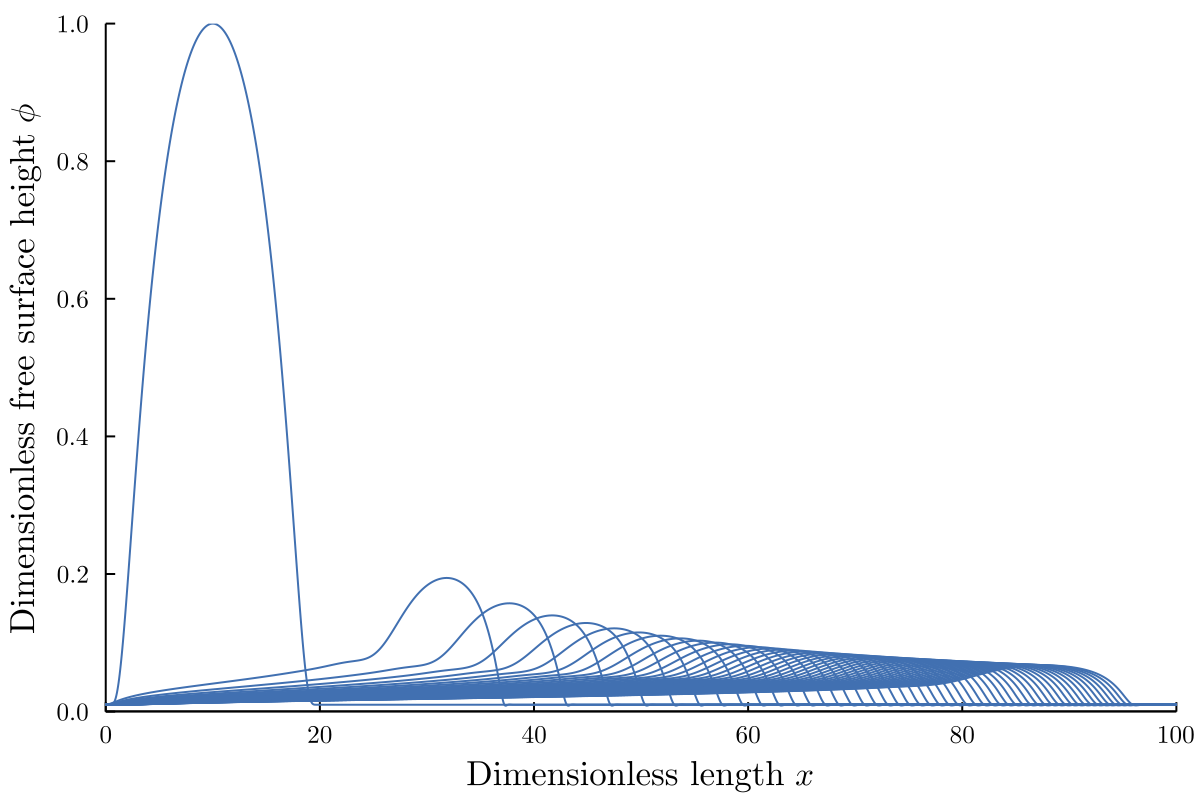
\includegraphics[width=\textwidth]{images/flat/plt_notitle.png}
            \caption{Profile plot}
            \label{fig:drop_flat_profile}
        \end{subfigure}%
        \begin{subfigure}[ht]{.5\textwidth}
            
\includegraphics[width=\textwidth]{images/placeholder.png}
            \caption{Profile animation}
            \label{fig:drop_flat_anim}
        \end{subfigure}
        \caption{Fluid profile for a drop initial condition with a flat topography} 
    \end{figure}
\end{frame} 
\begin{frame}
    \begin{figure}
        \centering
        \begin{subfigure}[ht]{.5\textwidth}
            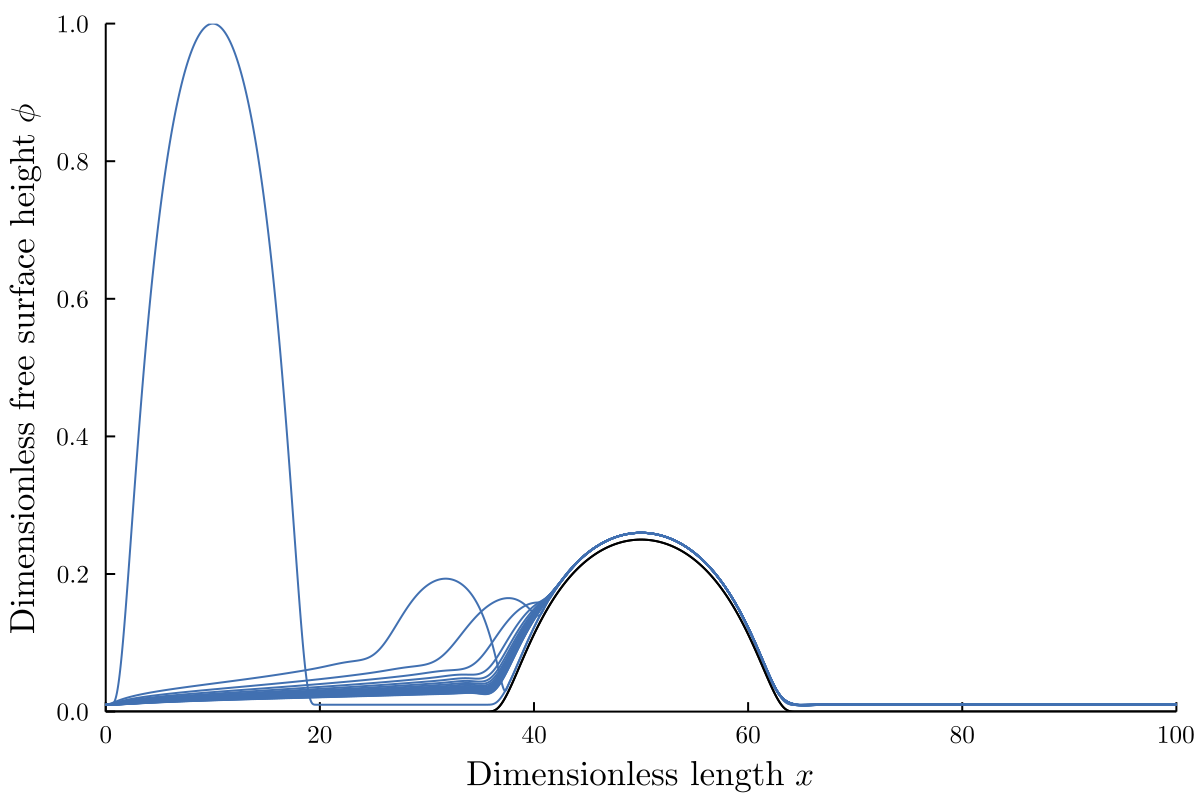
\includegraphics[width=\textwidth]{images/bump_25_shorter/plt_notitle.png}
            \caption{Profile plot}
            \label{fig:drop_25_profile}
        \end{subfigure}%
        \begin{subfigure}[ht]{.5\textwidth}
            
\includegraphics[width=\textwidth]{images/placeholder.png}
            \caption{Profile animation}
            \label{fig:drop_25_anim}
        \end{subfigure} 
        \caption{Fluid profile for a drop initial condition with a bump topography of height 0.25} 
    \end{figure}
\end{frame} 
\begin{frame}
    \begin{figure}
        \centering
        \begin{subfigure}[ht]{.5\textwidth}
            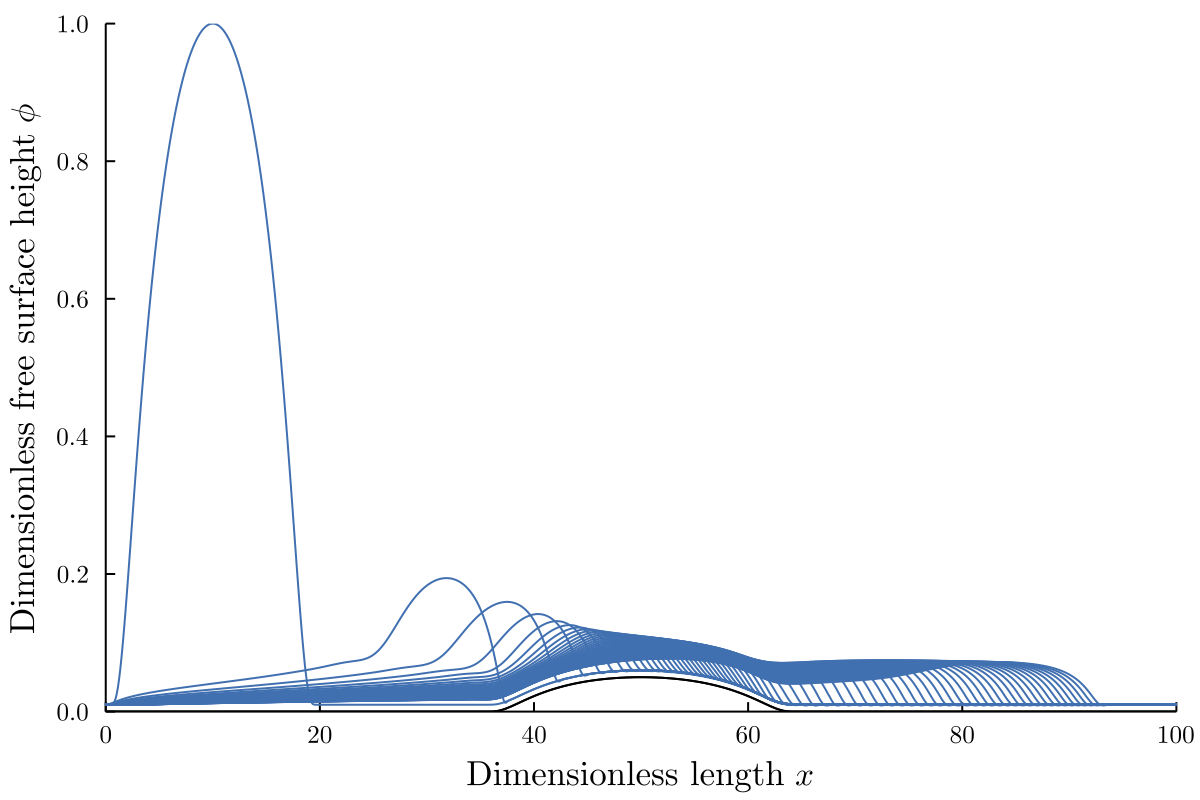
\includegraphics[width=\textwidth]{images/bump_10/plt_notitle.png}
            \caption{Profile plot}
            \label{fig:drop_10_profile}
        \end{subfigure}%
        \begin{subfigure}[ht]{.5\textwidth}
            
\includegraphics[width=\textwidth]{images/placeholder.png}
            \caption{Profile animation}
            \label{fig:drop_10_anim}
        \end{subfigure}
        \caption{Fluid profile for a drop initial condition with a bump topography of height 0.10} 
    \end{figure}
\end{frame} 